\documentclass[12pt,a4paper]{article}
\usepackage[margin=1in]{geometry}
\usepackage{ctex}
\usepackage{amsmath}
\usepackage{setspace}
\usepackage{fancyhdr}
\usepackage{lastpage}
% 关键：设置英文数字为 Times New Roman
\usepackage{fontspec}
%\setmainfont{Times New Roman}
\setCJKmainfont{SimSun} % 中文保持宋体
\usepackage{graphicx}%图片
\usepackage{xcolor}%颜色
\usepackage{listings}%支持代码
\lstset{
	language=C,
	basicstyle=\ttfamily\small,%字体样式
	keywordstyle=\color{blue},%关键字颜色
	commentstyle=\color{gray}, %注释颜色
	numbers=left,%行号位置
	numberstyle=\tiny\color{gray},%行号样式
	frame=single,%边框样式
	showspaces=false, %不显示空格标记
	showstringspaces=false,%不显示字符串中的空格标记
	inputencoding=utf8,%输入编码
	extendedchars=true%支持拓展字符
}


% 页面设置
\geometry{a4paper,left=2.5cm,right=2.5cm,top=2.5cm,bottom=2.5cm}
\onehalfspacing

% 页眉页脚
\pagestyle{fancy}
\fancyhf{}
\lhead{江西财经大学}
\rhead{C++综合实践实训报告}
\cfoot{第 \thepage\ 页 / 共 \pageref{LastPage} 页}

\begin{document}
\thispagestyle{empty}
% 封面（优化版：固定下划线长度 + 居中文字 + 增大字号）
\begin{center}


    {\Huge \textbf{江西财经大学}}\\[1cm]
    {\Large \textbf{2025–2026 学年第 3 学期}}\\[1cm]
    {\LARGE \textbf{《C++综合实践》实训习题}}\\[2cm]

    \vspace{3cm}
{\zihao{4}
\makebox[2cm][s]{\songti 课程代码}\underline{\makebox[3.5cm][c]{ 1005405122}}\quad \makebox[2cm][s]{\songti 选课班}\underline{\makebox[3.5cm][c]{\songti 软工VR255班}}\\[0.5cm]
\makebox[2cm][s]{\songti 课程名称}\underline{\makebox[3.5cm][c]{ \songti C++综合实践}}\quad \makebox[2cm][s]{\songti 任课教师}\underline{\makebox[3.5cm][c]{\songti 张勇}}\\[0.5cm]
\makebox[2cm][s]{\songti 学号}\underline{\makebox[3.5cm][c]{ 0256658}}\quad \makebox[2cm][s]{\songti 姓名}\underline{\makebox[3.5cm][c]{\songti 桑赫}}\\[0.5cm]

\makebox[2cm][s]{\songti 学院}\quad\underline{\makebox[9cm][c]{\songti  虚拟现实(VR)现代产业学院}}\\[0.5cm]
\makebox[2cm][s]{\songti 专业}\quad\underline{\makebox[9cm][c]{\songti  软件工程(VR软件开发)}}\\[0.5cm]
}

    \vspace{2cm}
    {\large 2026 年 6 月 14 日}
\end{center}

\newpage


% 实训题1
\section*{实训题1}
设有4个学生，每个学生有5门课的成绩，要求从键盘输入学生的学号、姓名及5门课的成绩，计算出平均成绩，并将每个学生的全部数据以字符串的形式保存到磁盘上的文本文件StudentGrade.txt中。



\begin{lstlisting}[language=C]

#include<iostream>
using namespace std;
#include<string>
#include<iomanip>
#include<cstdlib>
#include<fstream>
#include<sstream>

class Student{
private:    
string m_name;
    int m_id;
    int grades[5];
    double m_average;

    public:
    
       void input(){
        cout<<"请输入学生姓名："<<endl;
        cin>>m_name;
        this->m_name;
        cout<<"请输入学生学号："<<endl;
        cin>>m_id;
        this->m_id;
      
        int sum=0;
        for(int i=0;i<5;i++){
            cout<<"请输入第"<<i+1<<"门课程成绩："<<endl;
            cin>>this->grades[i];
            sum+=this->grades[i];
        }
        this->m_average=(double)sum/5;}

      string toString() const {
        ostringstream oss;
        oss << m_name << "；" << m_id;
        for(int i = 0; i < 5; i++) {
            oss << "；" << grades[i];
        }
        oss << "；" << fixed << setprecision(2) << m_average;
        return oss.str();
      }

      void write(){
        ofstream ofs("StudentGrade.txt", ios::app);
        if(!ofs) {
            cerr << "无法打开文件 StudentGrade.txt" << endl;
            return;
        }
        ofs << toString() << endl;

        ofs.close();
      }

   
};
int main(){
    system("chcp 65001 > nul");

    for(int i = 0; i < 4; i++){
      cout << "输入第" << i+1 << "位学生信息" << endl;
      Student s;
      s.input();
      s.write();
    }

  return 0;
}


\end{lstlisting}


\begin{figure}[h]
\centering%图片居中
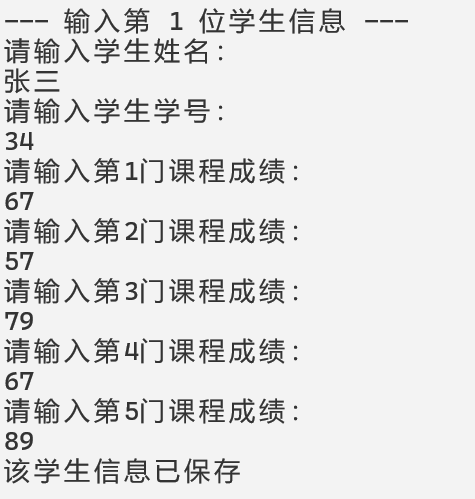
\includegraphics[width=0.7\textwidth]{1.png}
\caption{实验一运行结果}
\label{result}

\end{figure}







\vspace*{\fill}
\newpage

% 实训题2
\section*{实训题2}
读取上题中的文本文件StudentGrade.txt中的数据，按平均成绩进行降序排序，并将排序后的所有数据保存到新的文本文件SortedGrade.txt中。

\textbf{提示：}所有学生的数据保存到字符串数组中，字符串数组的每个元素是一个字符串，包含了一个学生的所有数据，平均成绩应该是出现在第7个;号到本行结束之间的所有字符，读出平均成绩，按成绩对字符串数组排序。
\begin{lstlisting}[language=C]
#include<iostream>
#include<string>
#include<iomanip>
#include<cstdlib>
#include<fstream>
#include<vector>
#include<algorithm>

using namespace std;

static double extractAverage(const string &line) {
    const char delimiter = '；';
    int count = 0;
    size_t pos = string::npos;
    for(size_t i = 0; i < line.size(); i++) {
        if(line[i] == delimiter) {
            count++;
            if(count == 7) {
                pos = i;
                break;
            }
        }
    }
    if(pos == string::npos || pos + 1 >= line.size()) {
        return 0.0;
    }
    string avgStr = line.substr(pos + 1);
    try {
        return stod(avgStr);
    } catch(...) {
        return 0.0;
    }
}

int main() {
    system("chcp 65001 > nul");

    vector<string> records;
    ifstream ifs("StudentGrade.txt");
    if(!ifs) {
        cerr << "无法打开文件 StudentGrade.txt" << endl;
        return 1;
    }

    string line;
    while(getline(ifs, line)) {
        if(!line.empty()) {
            records.push_back(line);
        }
    }
    ifs.close();

    sort(records.begin(), records.end(), [](const string &a, const string &b) {
        return extractAverage(a) > extractAverage(b);
    });

    ofstream ofs("SortedGrade.txt", ios::out);
    if(!ofs) {
        cerr << "无法创建文件 SortedGrade.txt" << endl;
        return 1;
    }

    for(const auto &record : records) {
        ofs << record << endl;
    }
    ofs.close();

    cout << "排序完成，结果已保存到 SortedGrade.txt" << endl;
    return 0;
}

\end{lstlisting}

\begin{figure}[h]
\centering%图片居中
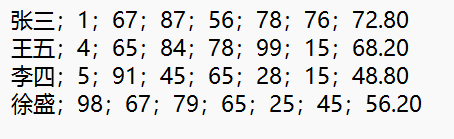
\includegraphics[width=0.7\textwidth]{2.png}
\caption{实验二运行结果}
\label{result}

\end{figure}
\vspace*{\fill}
\newpage

% 实训题3
\section*{实训题3}
构造结构体StudentGrade，要求从键盘输入学生的学号、姓名及5门课的成绩，计算出平均成绩，写入数据到结构体数组中。并将每个学生的全部数据保存到磁盘上的二进制文件StudentGrade.dat中。

\textbf{提示：}二进制文件创建语句pf=fopen("student.dat","wb");\par
写二进制文件语句fwrite(\&stu[i],sizeof(Student),1,fp);
\begin{lstlisting}[language=C]
#include <iostream>
#include <cstdio>
#include <cstring>
using namespace std;

struct StudentGrade {
    int id;
    char name[64];
    int scores[5];
    double average;
};

int main() {
    system("chcp 65001 > nul");

    int n;
    cout << "请输入学生数量：";
    cin >> n;
    if(n <= 0) {
        cerr << "学生数量必须大于0。" << endl;
        return 1;
    }
    if(n > 100) {
        cerr << "最大支持100名学生。" << endl;
        return 1;
    }

    StudentGrade *students = new StudentGrade[n];

    for(int i = 0; i < n; i++) {
        cout << "\n请输入第" << i + 1 << "名学生的学号：";
        cin >> students[i].id;
        cout << "请输入第" << i + 1 << "名学生的姓名：";
        cin >> students[i].name;
        int sum = 0;
        for(int j = 0; j < 5; j++) {
            cout << "请输入第" << i + 1 << "名学生第" 
			<< j + 1 << "门成绩：";
            cin >> students[i].scores[j];
            sum += students[i].scores[j];
        }
        students[i].average = static_cast<double>(sum) / 5.0;
    }

    FILE *fp = fopen("StudentGrade.dat", "wb");
    if(!fp) {
        cerr << "无法创建二进制文件 StudentGrade.dat" << endl;
        delete[] students;
        return 1;
    }

    for(int i = 0; i < n; i++) {
        fwrite(&students[i], sizeof(StudentGrade), 1, fp);
    }

    fclose(fp);
    delete[] students;
    cout << "已将 " << n << " 名学生的全部数据保存到 StudentGrade.dat" 
	<< endl;
    return 0;
}

\end{lstlisting}
\begin{figure}[h]
\centering%图片居中
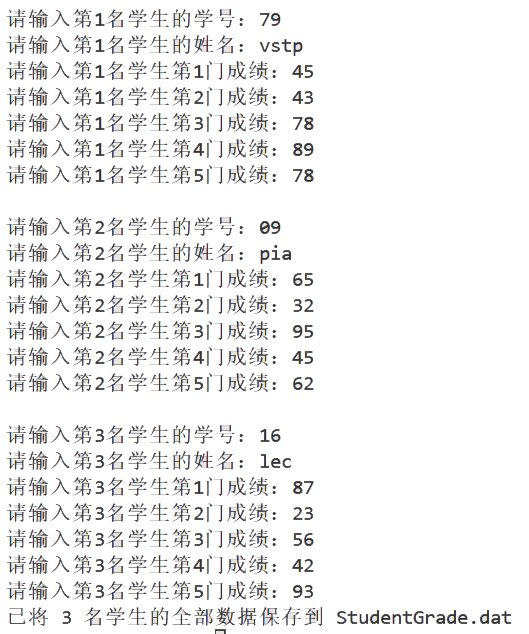
\includegraphics[width=0.7\textwidth]{3.png}
\caption{实验三运行结果}
\label{result}
\end{figure}
\vspace*{\fill}








\newpage

% 实训题4
\section*{实训题4}
设计一个函数SortByAvg()，读取上题中的二进制文件StudentGrade.dat中的数据到结构体数组中，按平均成绩进行降序排序，并将排序后的所有数据保存到新的二进制文件SortedGrade.dat中。
\begin{lstlisting}[language=C]
#include<iostream>
#include<cstdio>
#include<cstring>
#include<algorithm>
using namespace std;

struct StudentGrade {
	int id;
	char name[64];
	int scores[5];
	double average;
};

void SortByAvg(const char *inFile = "StudentGrade.dat", 
const char *outFile = "SortedGrade.dat"){
	FILE *fp = fopen(inFile, "rb");
	if(!fp){
		cerr << "无法打开输入文件 " << inFile << endl;
		return;
	}
	if(fseek(fp, 0, SEEK_END) != 0){ fclose(fp); 
	cerr << "读取文件长度失败" << endl; return; }
	long sz = ftell(fp);
	if(sz <= 0){ fclose(fp); 
	cerr << "输入文件为空或无法读取大小" << endl; return; }
	size_t count = static_cast<size_t>(sz / sizeof(StudentGrade));
	rewind(fp);

	StudentGrade *arr = new StudentGrade[count];
	size_t read = fread(arr, sizeof(StudentGrade), count, fp);
	fclose(fp);
	if(read == 0){ cerr << "未读取到任何记录" << endl;
	 delete[] arr; return; }

	sort(arr, arr + count, []
	(const StudentGrade &a, const StudentGrade &b)
	{ return a.average > b.average; });

	FILE *ofp = fopen(outFile, "wb");
	if(!ofp){ cerr << "无法创建输出文件 " << outFile << endl;
	 delete[] arr; return; }
	fwrite(arr, sizeof(StudentGrade), count, ofp);
	fclose(ofp);
	delete[] arr;
	cout << "已将排序后的数据保存到 " << outFile << endl;
}

int main(){
    system("chcp 65001 > nul");
	SortByAvg();
	return 0;
}
\end{lstlisting}
\begin{figure}[h]
\centering%图片居中
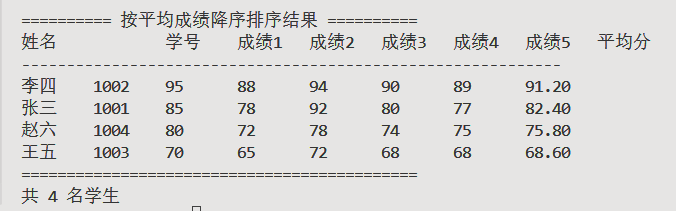
\includegraphics[width=0.7\textwidth]{4.png}
\caption{实验四运行结果}
\label{result}
\end{figure}
\vspace*{\fill}
\newpage

% 实训题5
\section*{实训题5}
编写一个随机加分的程序，要求如下：

(1) 事先编辑好一个存放所有学生学号的文本文件，每个学生的学号占一行, 假设总行数为m；

(2) 产生一个随机数$n(1<=n<=m)$，据此读取文本文件中的第n行的学生学号并输出，然后删除这个文本文件的第n行, 设置总行数为m -1；

(3) 在学生结构体数组中查询刚才随机挑选的学号的学生记录是否存在，如果存在则将该生的数学成绩加10分，并更新磁盘上的数据文件，如果不存在则提示查无此人。

(4) 将该功能实现为循环模式，可用户决定是否继续随机加分。

\textbf{解答：}
\begin{lstlisting}[language=C]
#include <iostream>
#include <fstream>
#include <vector>
#include <string>
#include <cstdlib>
#include <ctime>
#include <cstdio>
#include <cstring>
using namespace std;

struct StudentGrade {
    int id;
    char name[64];
    int scores[5];
    double average;
};

static bool readIdLines(const string &file, vector<string> &lines){
    lines.clear();
    ifstream ifs(file);
    if(!ifs) return false;
    string ln;
    while(getline(ifs, ln)){
        if(!ln.empty()) lines.push_back(ln);
    }
    return true;
}

static bool writeIdLines(const string &file,
 const vector<string> &lines){
    ofstream ofs(file, ios::out | ios::trunc);
    if(!ofs) return false;
    for(size_t i=0;i<lines.size();++i) ofs << lines[i] << "\n";
    return true;
}

static bool loadStudents(const char *file, vector<StudentGrade> &arr){
    arr.clear();
    FILE *fp = fopen(file, "rb");
    if(!fp) return false;
    if(fseek(fp, 0, SEEK_END) != 0){ fclose(fp); return false; }
    long sz = ftell(fp);
    if(sz <= 0){ fclose(fp); return false; }
    size_t count = static_cast<size_t>(sz / sizeof(StudentGrade));
    rewind(fp);
    arr.resize(count);
    size_t read = fread(arr.data(), sizeof(StudentGrade), count, fp);
    fclose(fp);
    return read == count;
}

static bool saveStudents(const char *file,
 const vector<StudentGrade> &arr){
    FILE *fp = fopen(file, "wb");
    if(!fp) return false;
    size_t written = fwrite(arr.data(), 
	sizeof(StudentGrade), arr.size(), fp);
    fclose(fp);
    return written == arr.size();
}

int main(){
    system("chcp 65001 > nul");
    const string idFile = "StudentIDs.txt"; // 每行一个学号
    const char *binFile = "StudentGrade.dat";

    srand((unsigned)time(NULL));

    while(true){
        vector<string> ids;
        if(!readIdLines(idFile, ids)){
            cerr << "无法打开或读取文件 " << idFile << endl;
            return 1;
        }
        size_t m = ids.size();
        if(m == 0){
            cout << "学号文件为空，退出。" << endl;
            break;
        }
        size_t n = (rand() % m); // 0-based index
        string chosen = ids[n];
        cout << "随机抽取到的学号：" << chosen << endl;

        ids.erase(ids.begin() + n);
        if(!writeIdLines(idFile, ids)){
            cerr << "删除行后无法写回学号文件" << endl;
            return 1;
        }

        vector<StudentGrade> students;
        if(!loadStudents(binFile, students)){
            cerr << "无法读取二进制学生文件或文件不存在：" << binFile 
			<< endl;
  
            break;
        }
        int targetId = 0;
        try{
            targetId = stoi(chosen);
        }catch(...){
            cerr << "学号不是有效整数：" << chosen << endl;

            cout << "是否继续随机加分？(y/n): ";
            string ans; cin >> ans; if(ans!="y" && ans!="Y") break; 
			else continue;
        }

        bool found = false;
        for(size_t i=0;i<students.size();++i){
            if(students[i].id == targetId){
                cout << "找到学号 " << targetId 
				<< "，原数学成绩：" 
				<< students[i].scores[0] << endl;
                students[i].scores[0] += 10;
                cout << "加分后数学成绩：" 
				<< students[i].scores[0] << endl;
  
                int sum = 0;
                for(int k=0;k<5;++k) sum += students[i].scores[k];
                students[i].average = static_cast<double>(sum) / 5.0;
                found = true;
                break;
            }
        }

        if(found){
            if(!saveStudents(binFile, students)){
                cerr << "无法将更新后的学生数据写回二进制文件" << endl;
                return 1;
            }
            cout << "已更新二进制文件中的成绩。" << endl;
        }else{
            cout << "查无此人（学号 " << targetId << "）。" << endl;
        }

        cout << "是否继续随机加分？(y/n): ";
        string ans; cin >> ans;
        if(ans != "y" && ans != "Y") break;
    }

    cout << "程序结束。" << endl;
    return 0;
}

\end{lstlisting}

\begin{figure}[h]
\centering%图片居中
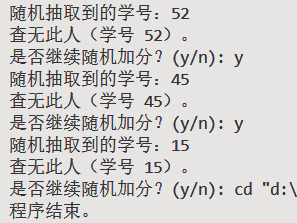
\includegraphics[width=0.7\textwidth]{5.png}
\caption{实验五运行结果}
\label{result}

\end{figure}






\vspace*{\fill}
\newpage

% 实训题6
\section*{实训题6}
修改学生结构体，增加籍贯和专业字段，并实现以下统计功能：

(1) 计算和报告各门课程按籍贯或按专业分组后成绩的最大值、最小值、均值、中位数。

(2) 按成绩统计，计算和报告各门课程各成绩段人数占选课人数的百分比。成绩分为5段：0、(0,60)、[60,75)、[75,90)、[90,100]。
\begin{lstlisting}[language=C]
#include <iostream>
#include <cstdio>
#include <cstring>
#include <vector>
#include <string>
#include <map>
#include <array>
#include <algorithm>
#include <cmath>
#include <iomanip>
using namespace std;

struct StudentGrade {
    int id;
    char name[64];
    char hometown[64];
    char major[64];
    int scores[5];
    double average;
};

static double calculateAverage(const StudentGrade &stu) {
    int sum = 0;
    for(int i = 0; i < 5; i++) sum += stu.scores[i];
    return static_cast<double>(sum) / 5.0;
}

static bool saveStudents(const char *file, 
const vector<StudentGrade> &students) {
    FILE *fp = fopen(file, "wb");
    if(!fp) return false;
    fwrite(students.data(),
	 sizeof(StudentGrade), students.size(), fp);
    fclose(fp);
    return true;
}

static bool loadStudents(const char *file, 
vector<StudentGrade> &students) {
    students.clear();
    FILE *fp = fopen(file, "rb");
    if(!fp) return false;
    if(fseek(fp, 0, SEEK_END) != 0) { fclose(fp); return false; }
    long sz = ftell(fp);
    if(sz <= 0) { fclose(fp); return false; }
    size_t count = static_cast<size_t>(sz / sizeof(StudentGrade));
    rewind(fp);
    students.resize(count);
    size_t readCount = fread(students.data(), 
	
	sizeof(StudentGrade), count, fp);
    fclose(fp);
    return readCount == count;
}

static double medianValue(vector<int> &values) {
    if(values.empty()) return 0.0;
    sort(values.begin(), values.end());
    size_t n = values.size();
    return (n % 2 == 1)
        ? static_cast<double>(values[n/2])
        : (static_cast<double>(values[n/2 - 1]) + 
		static_cast<double>(values[n/2])) / 2.0;
}


static void reportGroupStatistics(const vector<StudentGrade> &students, 
bool byHometown) {
    const char *groupName = byHometown ? "籍贯" : "专业";
    map<string, array<vector<int>, 5>> groupScores;

    for(const auto &stu : students) {
        string key = byHometown ? string(stu.hometown) : 
		string(stu.major);
        for(int i = 0; i < 5; i++) {
            groupScores[key][i].push_back(stu.scores[i]);
        }
    }

    cout << "\n按" << groupName << "分组的课程成绩统计：" << endl;
    for(const auto &entry : groupScores) {
        const string &key = entry.first;
        cout << "\n" << groupName << ": " << key << endl;
        cout << left << setw(12) << "课程" << setw(8) << "最小" 
		<< setw(8) << "最大" << setw(10) << "均值" << setw(10)
		 << "中位数" << "\n";
        for(int c = 0; c < 5; c++) {
            const vector<int> &values = entry.second[c];
            if(values.empty()) continue;
            vector<int> sorted = values;
            sort(sorted.begin(), sorted.end());
            int minv = sorted.front();
            int maxv = sorted.back();
            double sum = 0.0;
            for(int score : sorted) sum += score;
            double mean = sum / sorted.size();
            double med = medianValue(sorted);
            cout << left << setw(12) << ("Course" + to_string(c + 1))
                 << setw(8) << minv
                 << setw(8) << maxv
                 << setw(10) << fixed << setprecision(2) << mean
                 << setw(10) << fixed << setprecision(2) << med
                 << "\n";
        }
    }
}

static void reportGradeSegments(const vector<StudentGrade> &students) {
    const int courseCount = 5;
    const int segmentCount = 5;
    vector<array<int, segmentCount>> counts(courseCount);
    for(auto &arr : counts) arr.fill(0);

    for(const auto &stu : students) {
        for(int c = 0; c < courseCount; c++) {
            int score = stu.scores[c];
            if(score == 0) counts[c][0]++;
            else if(score > 0 && score < 60) counts[c][1]++;
            else if(score >= 60 && score < 75) counts[c][2]++;
            else if(score >= 75 && score < 90) counts[c][3]++;
            else if(score >= 90 && score <= 100) counts[c][4]++;
        }
    }

    int total = static_cast<int>(students.size());
    cout << "\n各课程成绩段人数及占比：" << endl;
    cout << left << setw(12) << "课程";
    cout << setw(10) << "0" << setw(12) << "(0,60)" 
	<< setw(12) << "[60,75)" << setw(12) << "[75,90)" << setw(12)
	 << "[90,100]" << "\n";

    for(int c = 0; c < courseCount; c++) {
        cout << left << setw(12) << ("Course" + to_string(c + 1));
        for(int s = 0; s < segmentCount; s++) {
            int cnt = counts[c][s];
            double pct = total > 0 ? 
			(static_cast<double>(cnt) * 100.0 / total) 
			: 0.0;
            cout << setw((s == 0) ? 10 : 12) << 
		(to_string(cnt) + "(" + to_string
		((int)round(pct)) + "%)");
        }
        cout << "\n";
    }
}

int main() {
    system("chcp 65001 > nul");
    int n;
    cout << "请输入学生数量：";
    cin >> n;
    if(n <= 0) {
        cerr << "学生数量必须大于0。" << endl;
        return 1;
    }
    if(n > 100) {
        cerr << "最大支持100名学生。" << endl;
        return 1;
    }

    vector<StudentGrade> students;
    students.reserve(n);
    for(int i = 0; i < n; i++) {
        StudentGrade stu;
        cout << "\n请输入第" << i + 1 << "名学生的学号：";
        cin >> stu.id;
        cout << "请输入第" << i + 1 << "名学生的姓名：";
        cin >> stu.name;
        cout << "请输入第" << i + 1 << "名学生的籍贯：";
        cin >> stu.hometown;
        cout << "请输入第" << i + 1 << "名学生的专业：";
        cin >> stu.major;
        int sum = 0;
        for(int j = 0; j < 5; j++) {
            cout << "请输入第" << i + 1 << "名学生第"
			 << j + 1 << "门成绩：";
            cin >> stu.scores[j];
            sum += stu.scores[j];
        }
        stu.average = static_cast<double>(sum) / 5.0;
        students.push_back(stu);
    }

    const char *fileName = "StudentGrade.dat";
    if(!saveStudents(fileName, students)) {
        cerr << "无法创建二进制文件 " << fileName << endl;
        return 1;
    }
    cout << "已将 " << n << " 名学生的全部数据保存到 " 
	<< fileName << endl;

    vector<StudentGrade> loaded;
    if(!loadStudents(fileName, loaded)) {
        cerr << "无法读取二进制文件 " << fileName << endl;
        return 1;
    }

    reportGroupStatistics(loaded, true);  // 按籍贯
    reportGroupStatistics(loaded, false); // 按专业
    reportGradeSegments(loaded);

    return 0;
}

\end{lstlisting}
\begin{figure}[h]
\centering%图片居中
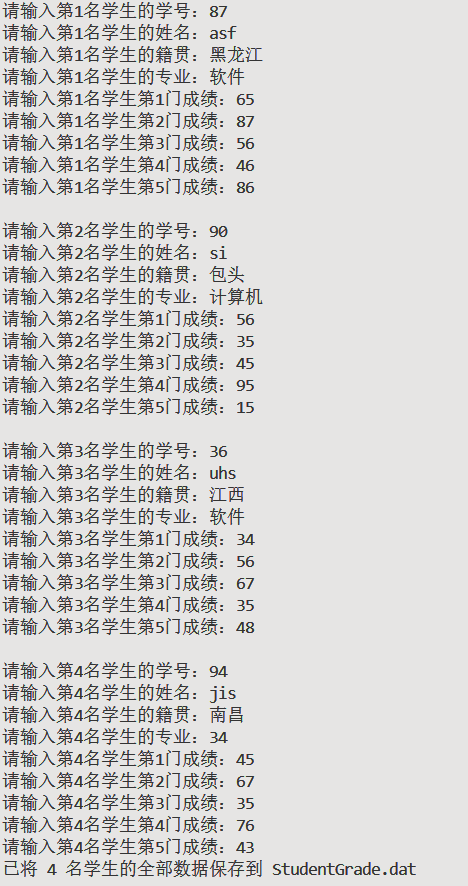
\includegraphics[width=0.7\textwidth]{61.png}
\caption{实验六运行结果}
\label{result}

\end{figure}
\begin{figure}[h]
\centering%图片居中
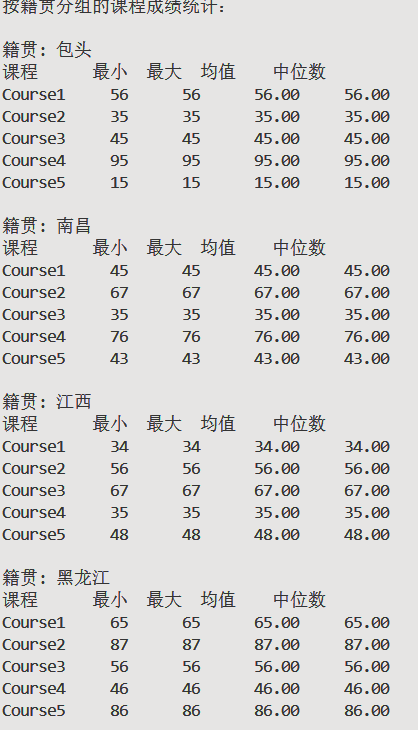
\includegraphics[width=0.7\textwidth]{62.png}
\caption{实验六运行结果}
\label{result}

\end{figure}
\begin{figure}[h]
\centering%图片居中
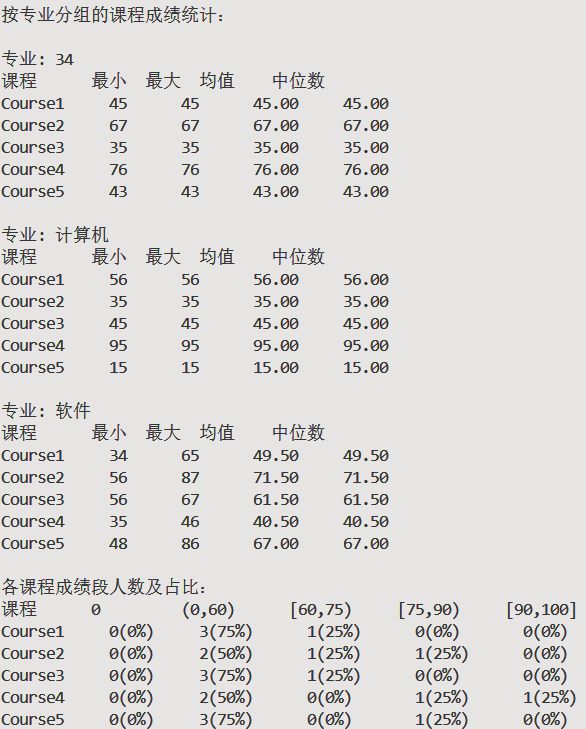
\includegraphics[width=0.7\textwidth]{63.png}
\caption{实验六运行结果}
\label{result}

\end{figure}
\vspace*{\fill}
\newpage

\end{document}